\newpage
\subsection{The power supply system}

\begin{figure}[!h]
    \centering
    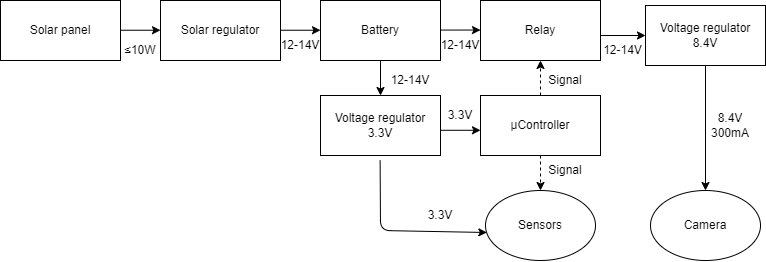
\includegraphics[width=0.8\textwidth]{\currfiledir/figures/alimentation_diagramme.png}
    \caption{Power supply architecture}
\end{figure}


\subsubsection{Camera and relay}
\begin{figure}[!h]
    \centering
    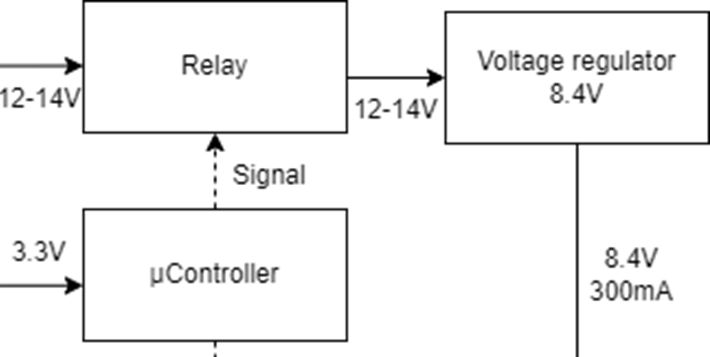
\includegraphics[width=0.5\textwidth]{\currfiledir/figures/camera_relay.png}
    \caption{Schematic showing the architecture of the camera and relay}
\end{figure}

The camera necessitates an 8.4V power supply and a current draw of 300mA for optimal operation. The system connects to the camera through a dummy battery featuring wired connections to the board. A relay, managed by the microcontroller, controls the camera's power supply. This approach is energy-efficient and offers low-power consumption. The relay consumes only 20mA of current when activated and no power when deactivated. Any relay with low power consumption operating at 3.3V is suitable for use.\\
To ensure voltage stability from the battery to the camera at 8.4V, a voltage regulator is placed after the relay. Installing the relay before the regulator helps avoid current loss within the regulator, enhancing the system's overall efficiency.



\begin{figure}[!h]
    \centering
    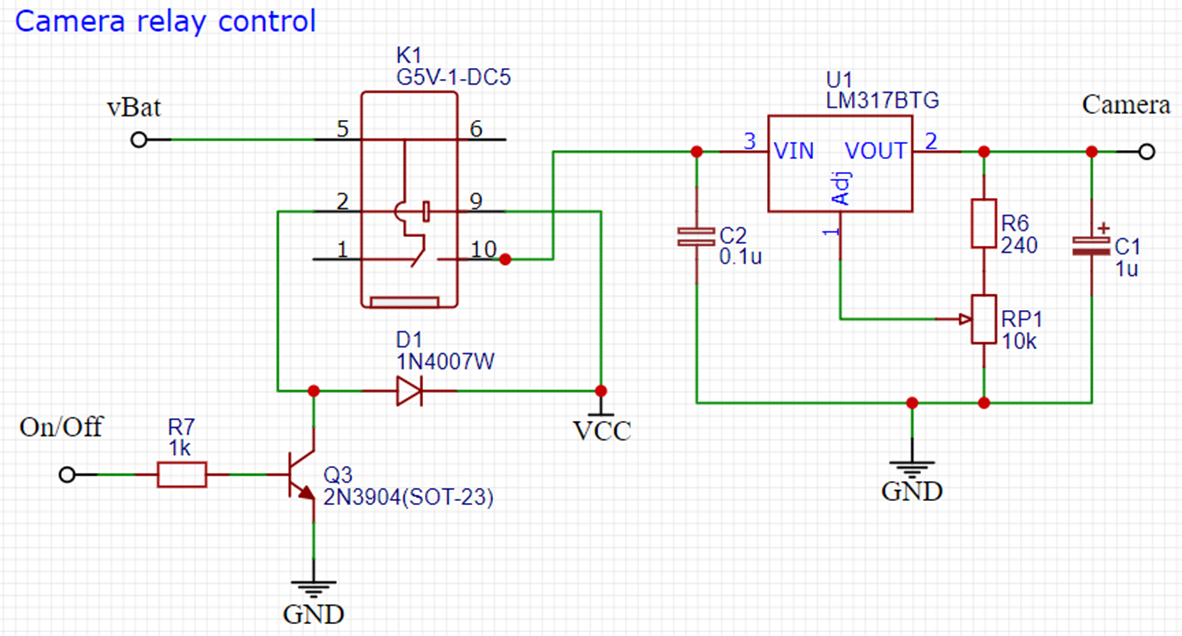
\includegraphics[width=1\textwidth]{\currfiledir/figures/relay.png}
    \caption{Camera-relay control}
\end{figure}

\newpage
\subsubsection{Battery and voltage regulator}

%Image avec sous figure
\begin{figure}[!h]
    \center{}
    %sous figure a
    \subfigure[Schematic showing the architecture of the regulator]{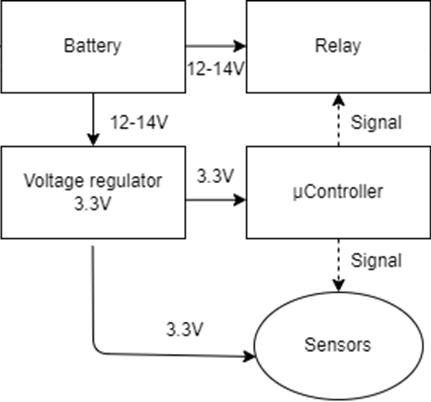
\includegraphics[width=0.4\textwidth]{\currfiledir/figures/regulator_33.png}}
    %sous figure b
    \subfigure[MT1763IS8 regulator]{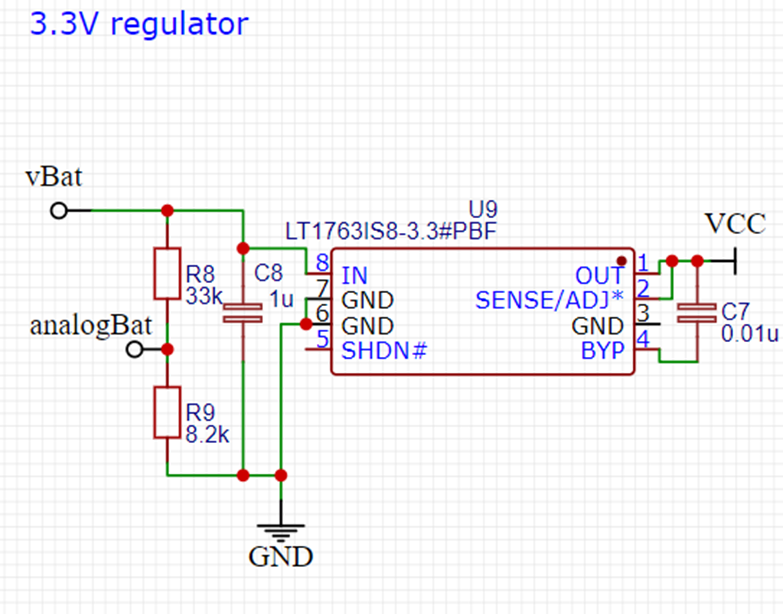
\includegraphics[width=0.59\textwidth]{\currfiledir/figures/regulator.png}}
    %légende de l'image
    % \caption{Exemple de sous-figure}
    %nom pour la citation de figure
\end{figure}
%fin de la figure

The LT1763IS8 is a voltage regulator designed to provide a stable 3.3V output while accepting an input voltage of up to 20V. It boasts a low quiescent current of 30µA, ensuring minimal power loss when supplying high output current, with less than 1mA lost to ground. Capable of delivering a maximum output current of 500mA, the LT1763IS8 is an efficient and reliable choice for regulating voltage in our application.

\newpage
\subsubsection{Sensors}
The system incorporates an array of low-power sensors, powered by a 3.3V voltage supply from the regulator, to ensure accurate and reliable measurements while maintaining low power consumption. These sensors are scheduled to collect data every 30 minutes and transmit the information through LoRa, with the exception of the motion sensor, which is read upon detecting an interruption. All data is also stored locally in a CSV format on a microSD card.\\
-	Motion Sensor: The ICM-20602 motion sensor operates in low power mode, consuming 1.33mA of current, and in Low-Noise mode, consuming 2.79mA. The primary purpose of the motion sensor is to detect when the container has been moved, which may cause the photos not to be aligned enough. When an interruption is detected, the motion sensor data, including rotation and acceleration, is read and transmitted through LoRa. The data format for motion is "date;gyro;acceleration".\\
-	Humidity/Temperature Sensor: The AM2320 sensor measures both humidity and external temperature, consuming 50µA in sleep mode and 1mA in active mode. The sensor reads data every 30 minutes and sends it through LoRa. The data format is "date;internal temperature;external temperature;humidity;light".\\
-	Internal Case Temperature Sensors: The LM35DZ sensors monitor the internal case temperature with a power consumption of less than 60µA. These sensors provide real-time data to the microcontroller.\\
-	Light Sensor: The TSL2561 light sensor operates with a power consumption of 2µA when turned down and a typical current of 0.24mA when active. This sensor measures ambient light levels every 30 minutes, and the light data is used to determine the lighting conditions when a photo is taken. If the light level at the scheduled photo-taking time is insufficient, the system will delay the photo-taking event until adequate lighting is available. The data format for this sensor is included in the combined format for the humidity/temperature sensor.\\
By using these low-power sensors, the system effectively minimizes energy consumption while still providing accurate and reliable measurements. All data, including sensor readings and motion events, is stored in a CSV format on a microSD card, ensuring that the information is readily available for analysis and review.

\subsubsection{Micro-controller}
The microcontroller used in the system is an STM32 Nucleo F303K8, which is powered at 3.3V directly from the voltage regulator. When active, with all peripherals disabled, it draws a current of 13mA. In sleep mode, with the Real-Time Clock (RTC) enabled, the microcontroller consumes only 3mA. It can be activated either by the interrupt signal from the motion detector or by the RTC at a predefined time, ensuring efficient power management and prolonging battery life while maintaining the responsiveness of the system. The STM32 Nucleo F303K8 offers flexible power options and low-power modes, making it suitable for energy-conscious applications that require optimal performance.

\newpage
% Solar panel and regulator
\subsubsection{Solar panel and regulator}
The primary power source for the system is a 12V 2.3Ah (27.6Wh) lead battery, chosen for its high capacity, its ability to retain charge over extended periods and its ability to resist to high temperatures. With an average power consumption of 127mAh a day, the battery can supply power up to 18 days.

\begin{table}[!h]
    \centering
    \begin{tabular}{|c|c|c|c|}
    \hline
     &
      \begin{tabular}[c]{@{}c@{}}Time where the system \\ is on per day(s)\end{tabular} &
      Current &
      \begin{tabular}[c]{@{}c@{}}Average consumption \\ per days (mAh)\end{tabular} \\ \hline
    Camera                     & 20    & 330 & 1,8333 \\ \hline
    Sensors                    & 480   & 50  & 6,6666 \\ \hline
    Sleep mode                 & 85900 & 5   & 119,30 \\ \hline
    Total consumption per days &       &     & 127,81 \\ \hline
    \end{tabular}
\end{table}

A 10W solar panel with 23\% efficiency is employed in this system to provide a significant safety margin, considering the intermittent nature of solar energy that can sometimes generate no power during the day. The solar panel is responsible for charging the lead battery during sunlight hours. A solar voltage regulator ensures that the voltage from the solar panel is within the appropriate range for charging the lead battery. The battery can be fully recharged with 2 days of sunshine.


\begin{figure}[!h]
    \centering
    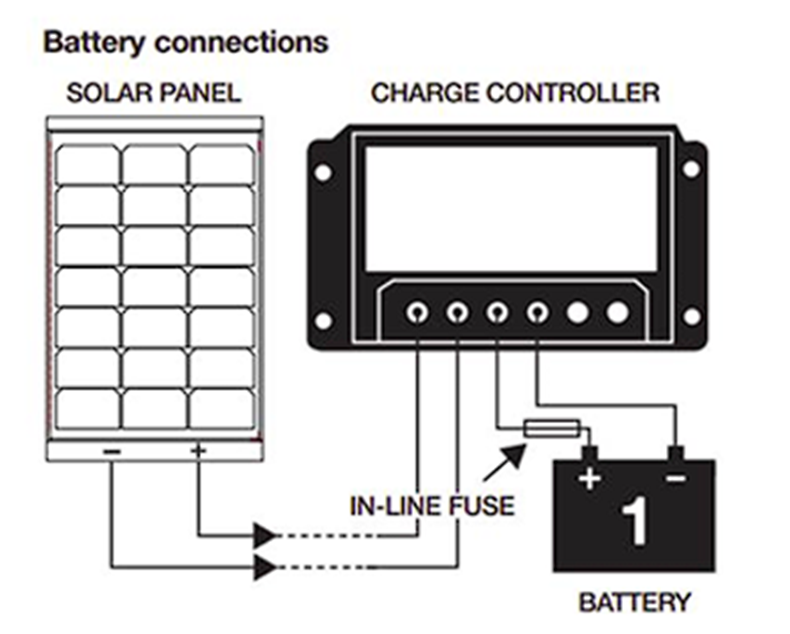
\includegraphics[width=0.8\textwidth]{\currfiledir/figures/battery_connection.png}
    \caption{Battery connection}
    \cite{battery}
\end{figure}

The solar panel and the battery are directly connected to the charge controller. The charge controller uses PWM to charge the battery with the good power.